\documentclass[journal]{IEEEtran}
\usepackage{amsmath, amsfonts, graphicx, listings, xcolor, float, subfig}

\definecolor{codegreen}{rgb}{0,0.6,0}
\definecolor{codegray}{rgb}{0.5,0.5,0.5}
\definecolor{codepurple}{rgb}{0.58,0,0.82}
\definecolor{backcolour}{rgb}{0.95,0.95,0.92}

\lstdefinestyle{mystyle}{
    backgroundcolor=\color{backcolour},   
    commentstyle=\color{codegreen},
    keywordstyle=\color{magenta},
    numberstyle=\tiny\color{codegray},
    stringstyle=\color{codepurple},
    basicstyle=\ttfamily\footnotesize,
    breakatwhitespace=false,         
    breaklines=true,                 
    captionpos=b,                    
    keepspaces=true,                 
    numbers=left,                    
    numbersep=5pt,                   
    showspaces=false,                
    showstringspaces=false,
    showtabs=false,                  
    tabsize=2
}

\lstset{style=mystyle}

\graphicspath{{./images/}}

\title{Lab 6: FIR Filtering of Nasal Air Temperature}
\author{
    \IEEEauthorblockN{Argenis Aquino, Rachel DuBois, Diego Lopez, Jonathan Sumner}
    \IEEEauthorblockA{
        Department of Engineering Technology, Rochester Institute of Technology\\
        1 Lomb Memorial Drive, Rochester, NY 14623, USA
    }
}

\begin{document}
\maketitle

\begin{abstract}
    This document demonstrates how an Arduino Uno was used to record analog temperature data by connecting it to an LM61 temperature sensor. The data from the temperature sensor was then used to measure nasal airflow temperature.
\end{abstract}

\section{Introduction}
\IEEEPARstart{A}{ir} flow temperature is higher when a person exhales and lower when they inhale.

\section{Methodology}
Section 1 focused on collecting and modeling real breathing temperature data for further analysis. The data, which exhibited a sinusoidal pattern with temperature drift, was either captured using MATLAB or provided in a pre-recorded dataset. The main goal was to estimate key parameters such as the linear drift slope, drift intercept, sinusoidal frequency, amplitude, and noise level.

The section began with the development of a MATLAB model, where recorded temperature data was analyzed, drift was removed, and breathing cycle characteristics were estimated. Once validated, the model was implemented in Arduino C, allowing the signal to be used as a controlled input for testing filtering techniques. Based on \texttt{CodeBase\_Lab06\_Section1\_2215.ino}, the Arduino sketch collected and processed 256 temperature sensor samples, converting ADC readings into temperature values.

A mathematical model of the breathing signal was created by simulating both drift and sinusoidal variation, with uniform noise empirically adjusted to match the real data. The final model was transferred to the Arduino, replacing real sensor data with a simulated breathing function to provide consistent testing conditions.

Validation involved comparing the simulated output with real sensor data and the MATLAB model. The system's responsiveness was optimized by adjusting the sampling rate (TSAMP\_MSEC) to speed up data collection without affecting the model's behavior.

Section 2 built upon the breathing model by exploring how temperature data can be represented using both floating-point and fixed-point formats. Floating-point temperature values were recorded and then scaled by factors of 1, 10, 100, and 1000 before being converted into fixed-point integers. This conversion introduced rounding errors, leading to quantization noise, which was quantified by computing the standard deviation of the error between the scaled floating-point and fixed-point values.

Using MATLAB, the system captured and analyzed the data. The noise levels were calculated by measuring the standard deviation of the quantization error, while signal strength was determined from the standard deviation of the scaled floating-point values. Comparative plots of fixed-point and floating-point representations helped visualize the effect of scaling on precision.

The risk of overflow in fixed-point representation was also considered when choosing scaling factors, ensuring that values remained within valid data type limits. This experiment demonstrated the advantages of fixed-point representation, which reduces memory usage and improves computational efficiency, especially in embedded systems where floating-point operations can be costly.

Section 3 implemented a moving average filter (MAV) to reduce sensor noise in the breathing signal. The input and output data were represented in centi-degrees Celsius by setting DATA\_FXPT = 100, ensuring consistent scaling. The effect of MAV kernel length on noise suppression and signal attenuation was analyzed, revealing the trade-offs between filtering performance and signal fidelity.

The Arduino code "CodeBase\_Lab06\_Section3\_2215.ino" was modified to generate filter coefficients for either a MAV or sinc FIR filter. These coefficients were displayed in the command window before data collection, allowing for verification of the filter parameters. In the main loop, a fixed-point temperature signal was simulated and convolved with the filter kernel, with input and output data captured in MATLAB for further analysis.

The filter's symmetry was investigated by adjusting the kernel size. The linear phase sinc kernel required an odd number of elements to maintain symmetry and ensure a well-defined impulse response. The experiment used MFILT = 11 and MFILT = 41, and the filter response was analyzed in MATLAB by plotting the input and output signals.

The filter’s transient response was also observed, noting expected distortion during the first MFILT samples due to buffer initialization in the convolution process. To improve visualization, early output samples were replaced with input values, making the filtered signal easier to compare. The impact of kernel length was assessed by plotting results for different MFILT values and evaluating changes in noise suppression and signal attenuation.

Section 4 enhanced the FIR filtering technique by introducing a windowed sinc filter to improve noise suppression, especially for high-frequency components. The procedure involved switching from a moving average filter (MAV) to a sinc filter with a corner frequency (Fc) set to 0.05, corresponding to a breathing rate of 30 breaths per minute. The filter kernel length, MFILT, was initially set to 11, and the effect of kernel length on output signal quality was analyzed by comparing input and output signals in MATLAB.

The filter’s DC gain was analyzed by calculating the sum of the kernel samples, ensuring a normalized output. The experiment demonstrated that the filter effectively isolated low-frequency breathing signals while attenuating high-frequency noise. The impact of kernel length on the number of valid output samples and the amplitude of both signal and noise components was explored with MFILT values of 11 and 41. MATLAB plots visually compared the input and output, showing that noise attenuation improved with increased kernel length.

Section 5 explored converting the sinc FIR filter from floating-point to fixed-point implementation, examining the speed advantages of integer arithmetic in embedded systems. The sinc filter kernel, initially computed in floating-point, was scaled and converted into fixed-point integers using a specified scale factor (HFXPT). The fixed-point convolution was implemented in Arduino C, where simulated temperature signals were processed by the fixed-point filter kernel.

The effect of fixed-point scaling on kernel values was examined, particularly the rounding errors that occurred during conversion, which resulted in some zero values in the fixed-point kernel. A minimum HFXPT value was determined to ensure all non-zero kernel elements remained greater than or equal to ±1. Additionally, the maximum value of the convolution sum before division by HFXPT was calculated for a 50°C DC input, considering whether the result could be represented using either float or long types.

To assess the accuracy of fixed-point computations, the error between floating-point and fixed-point kernel implementations was computed. The results highlighted the trade-offs between precision and computational efficiency, with fixed-point implementations offering faster execution and reduced memory usage, but with slightly higher errors compared to floating-point implementations.

\section{Results}

%%% Section 1 %%%
\begin{figure}[H]
    \centering
    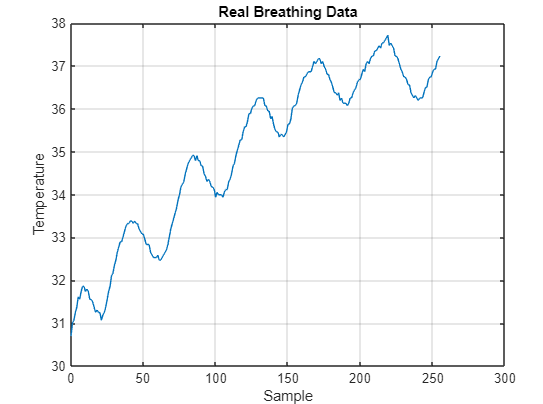
\includegraphics[width=\linewidth]{1.1.png}
    \caption{Real Breathing Data plot}
    \begin{minipage}{\linewidth}
        The MATLAB model successfully ploted the real breathing data. 
    \end{minipage}
    \label{fig:part1}
\end{figure}

\begin{figure}[H]
    \centering
    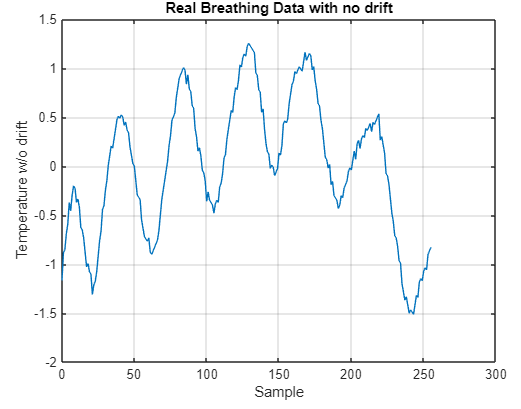
\includegraphics[width=\linewidth]{1.2.png}
    \caption{Real Breathing Data without Drift plot}
    \vspace{1em} % Adds vertical space
    \begin{minipage}{\linewidth}
        The MATLAB model successfully removed the drift component from the real breathing data, revealing the underlying sinusoidal pattern. The estimated parameters closely matched the real data, validating the model's accuracy: \( f(t) = A \sin(2\pi ft) + b \).
    \end{minipage}
    \label{fig:part1_noDrift}
\end{figure}

\begin{figure}[H]
    \centering
    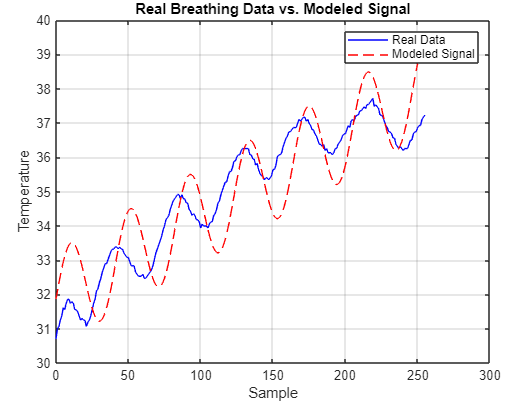
\includegraphics[width=\linewidth]{1.3.png}
    \caption{Real vs Modeled Breathing Data}
    \vspace{1em} % Adds vertical space
    % \begin{minipage}{\linewidth}
    % \end{minipage}
    \label{fig:part1_Comparison}
\end{figure}

%%% Section 2 %%%
\begin{figure}[H]
    \centering
    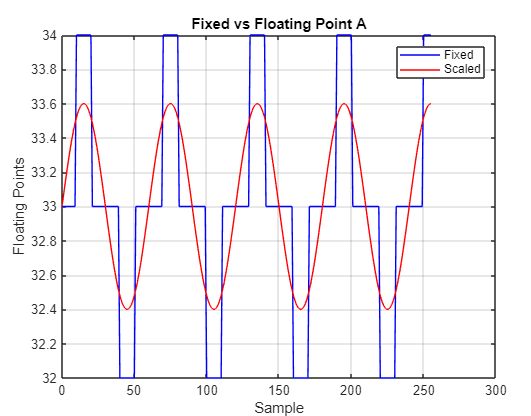
\includegraphics[width=\linewidth]{2.1.png}
    \caption{Fixed vs Floating Point A}
    % \begin{minipage}{\linewidth}
    % \end{minipage}
    \label{fig:part2A}
\end{figure}

\begin{figure}[H]
    \centering
    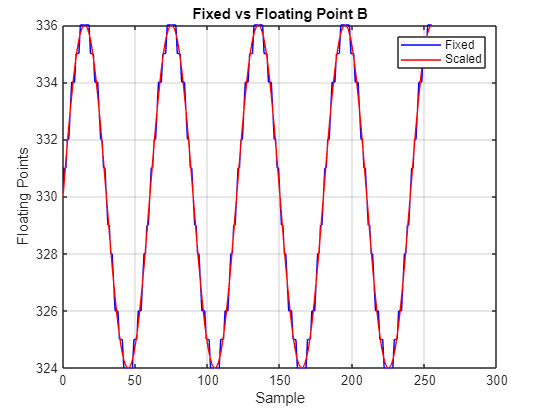
\includegraphics[width=\linewidth]{2.2.png}
    \caption{Fixed vs Floating Point B}
    % \begin{minipage}{\linewidth}
    % \end{minipage}
    \label{fig:part2B}
\end{figure}

\begin{figure}[H]
    \centering
    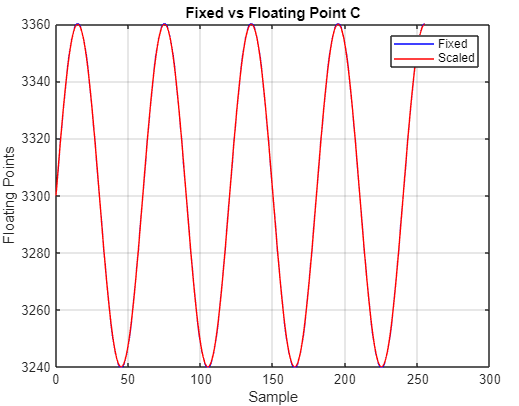
\includegraphics[width=\linewidth]{2.3.png}
    \caption{Fixed vs Floating Point C}
    \vspace{1em} % Adds vertical space
    % \begin{minipage}{\linewidth}
    % \end{minipage}
    \label{fig:part2C}
\end{figure}

\begin{figure}[H]
    \centering
    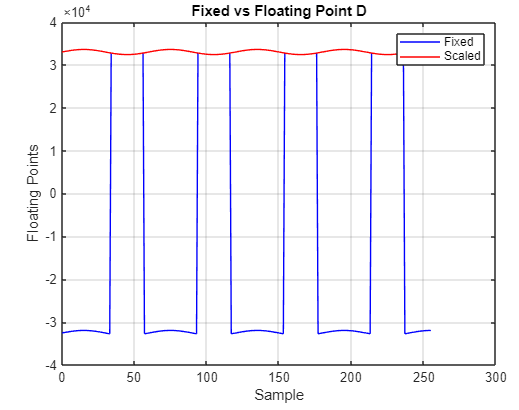
\includegraphics[width=\linewidth]{2.4.png}
    \caption{Fixed vs Floating Point D}
    % \begin{minipage}{\linewidth}
    % \end{minipage}
    \label{fig:part2D}
\end{figure}

%%% Section 3 %%%
\begin{figure}[H]
    \centering
    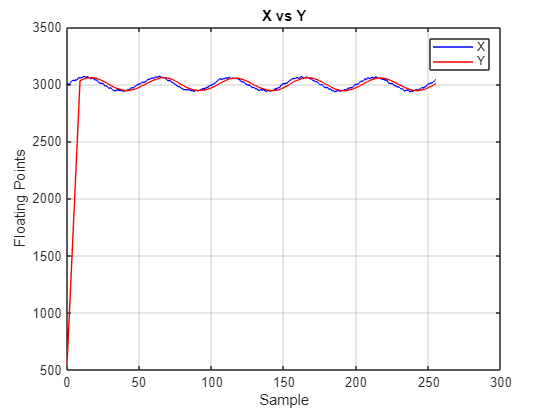
\includegraphics[width=\linewidth]{3.1.png}
    \caption{Fixed Point X vs Y A}
    % \begin{minipage}{\linewidth}
    % \end{minipage}
    \label{fig:part3A}
\end{figure}

\begin{figure}[H]
    \centering
    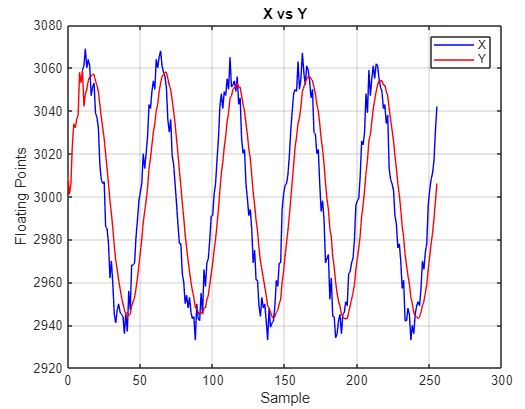
\includegraphics[width=\linewidth]{3.2.png}
    \caption{Fixed Point X vs Y B}
    % \begin{minipage}{\linewidth}
    % \end{minipage}
    \label{fig:part3B}
\end{figure}

\begin{figure}[H]
    \centering
    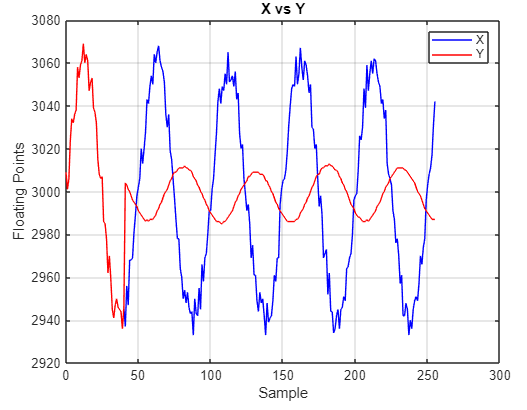
\includegraphics[width=\linewidth]{3.3.png}
    \caption{Fixed Point X vs Y C}
    \vspace{1em} % Adds vertical space
    % \begin{minipage}{\linewidth}
    % \end{minipage}
    \label{fig:part3C}
\end{figure}

%%% Section 4 %%%
\begin{figure}[H]
    \centering
    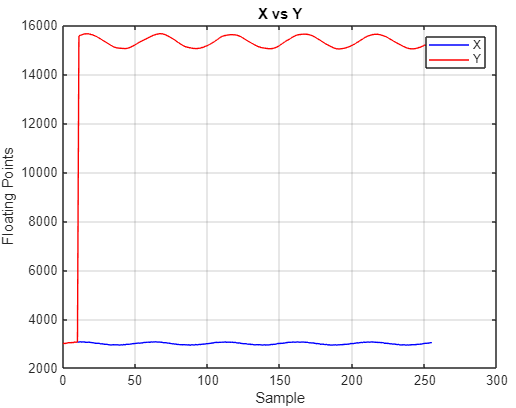
\includegraphics[width=\linewidth]{4.1.png}
    \caption{Windowed Sinc Filter}
    % \begin{minipage}{\linewidth}
    % \end{minipage}
    \label{fig:part4A}
\end{figure}

\begin{figure}[H]
    \centering
    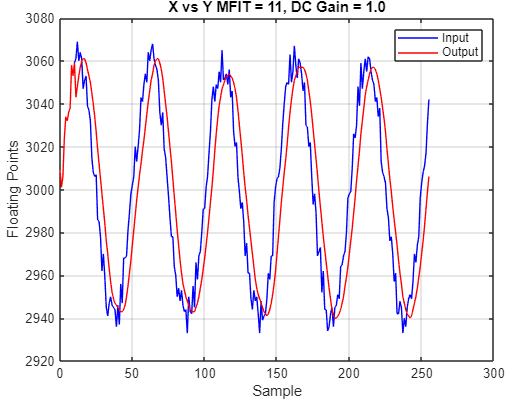
\includegraphics[width=\linewidth]{4.2.png}
    \caption{MFILT = 11}
    % \begin{minipage}{\linewidth}
    % \end{minipage}
    \label{fig:part4B}
\end{figure}

\begin{figure}[H]
    \centering
    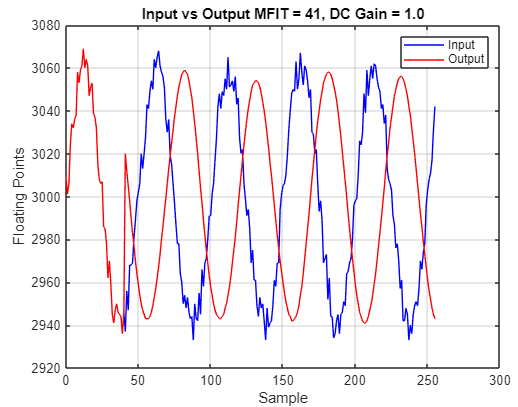
\includegraphics[width=\linewidth]{4.3.png}
    \caption{MFILT = 41}
    % \begin{minipage}{\linewidth}
    % \end{minipage}
    \label{fig:part4C}
\end{figure}

%%% Section 5 %%%
\begin{figure}[H]
    \centering
    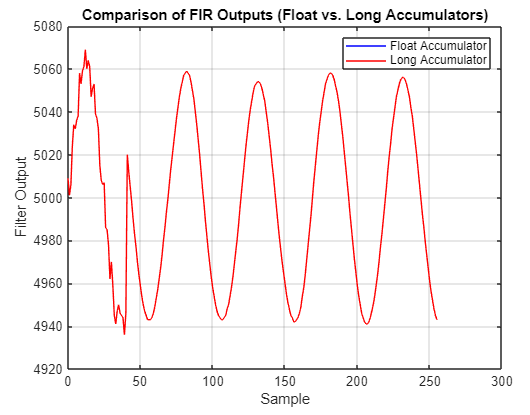
\includegraphics[width=\linewidth]{5.1.png}
    \caption{FIR Output Comparison}
    % \begin{minipage}{\linewidth}
    % \end{minipage}
    \label{fig:part5A}
\end{figure}

\begin{figure}[H]
    \centering
    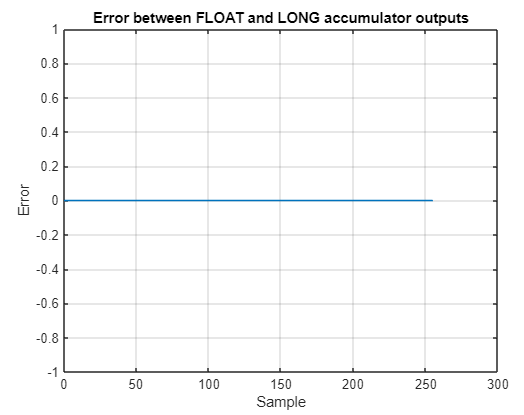
\includegraphics[width=\linewidth]{5.2.png}
    \caption{Float and Long Error Comparison}
    % \begin{minipage}{\linewidth}
    % \end{minipage}
    \label{fig:part5B}
\end{figure}

\section{Analysis}

The methodology employed in this lab involved several key components to collect and process nasal airflow temperature data. Initially, real breathing data was captured and modeled to identify the drift, sinusoidal frequency, and amplitude of the breathing cycle. The use of MATLAB allowed for data analysis and the removal of drift, ensuring a more accurate representation of the sinusoidal pattern in the data. Once the model was validated, it was implemented on the Arduino, and the system was used to simulate breathing signals for testing filtering techniques.

In Section 2, the conversion of floating-point to fixed-point data representation was explored, demonstrating how scaling impacts precision and memory usage. This approach highlighted the trade-offs between fixed-point and floating-point representations, with fixed-point offering advantages in memory efficiency but introducing quantization noise. This was verified through the standard deviation of the error between both formats.

Section 3’s use of a moving average filter (MAV) demonstrated the trade-offs between noise suppression and signal fidelity. The kernel length directly influenced the filter’s performance, with longer kernels providing better noise reduction at the expense of signal attenuation. In Section 4, a windowed sinc filter further enhanced noise suppression, particularly for high-frequency components, and showed the effect of kernel length on both noise reduction and valid output samples.

Finally, Section 5 focused on converting the sinc FIR filter to fixed-point implementation, which highlighted the computational advantages in embedded systems. The results showed that while fixed-point representation allowed faster execution and reduced memory usage, it introduced small errors due to rounding, which were more pronounced in the higher kernel lengths.

\section{Conclusion}

The experiments demonstrated the effectiveness of both fixed-point and floating-point representations for processing nasal airflow temperature data. Fixed-point representation, in particular, provided significant memory and computational efficiency, making it ideal for embedded systems. The moving average and windowed sinc filters were successful in reducing noise from the sensor data, with the windowed sinc filter offering better suppression of high-frequency noise. The analysis of the filter’s response and the conversion to fixed-point implementation showed the trade-offs between accuracy and system performance, making it evident that a balance must be struck between precision and computational resources. Overall, this study provides valuable insights into the design and implementation of efficient signal processing techniques for embedded systems.


\end{document}
